\subsection{Overview}

\begin{figure}[h]
    \centering
    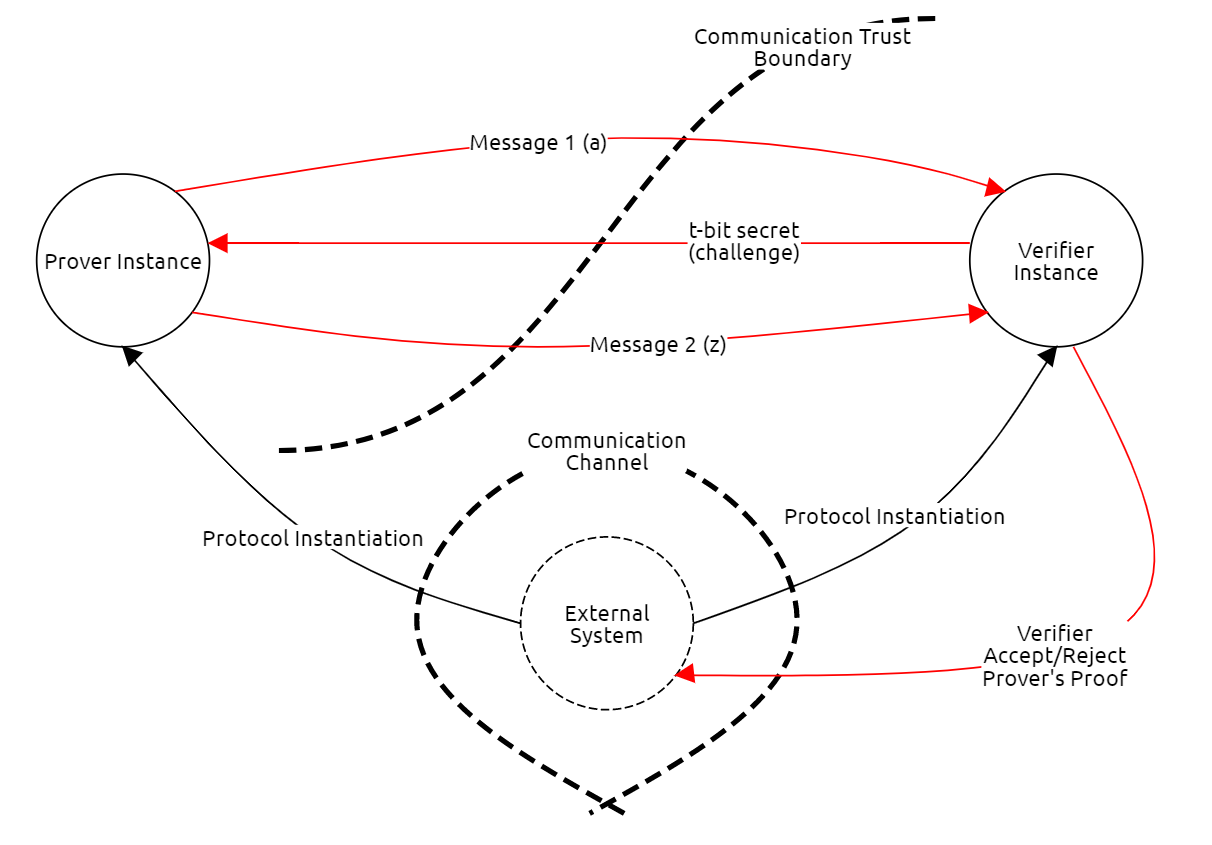
\includegraphics[width=\linewidth]{threat-model.png}
    \caption{Threat Model Diagram}
    \label{fig:threat_model}
\end{figure}

There should be no known way for adversaries to use the protocol in a way that it is not designed to. For example, under normal circumstances, the verifier should not have rewind access to a prover, this means that we will need to model state within the protocol and ensure that it is used properly (state-machine model). This should be a target of penetration tests. 


